\TODO

\subsection{Cellular Automata}

\begin{itemize}
    \item What is a Cellular Automata?
    \item Turing-complete CA with 29 states \cite{neumann1966selfreplication}.
    \item Codd: Turing-complete CA with 8 states, given some conditions \cite{codd1968cellular}
    \item Langton's research on emergent computation and phase transition \cite{langton1990edgeofchaos}.
    \item Wolfram's four qualitative CA classes \cite{wolfram1984complexity}?
\end{itemize}

\subsection{Self-Replication}

\begin{itemize}
    \item von Neumann's work on self-replication from around 1950 \cite{neumann1966selfreplication}.
    \item Self-replicating structures \cite{reggia1998neumann}
    \item Replicating universal computers with 63 states and 8500 rules \cite{perrier1996toward}.
\end{itemize}

\subsection{Evolution}

\begin{itemize}
    \item Genetic Algorithms
    \item Evolution in materio/silicon \cite{miller2014evolution}
\end{itemize}

\subsection{Artificial Development}

\begin{itemize}
    \item \cite{harding2008artificial} \cite{tufte2008evodevo}
    \item Zygote
    \item Scalability
    \item Robustness
    \item Plasticity
\end{itemize}

\subsection{Field Programmable Gate Array}

A Field Programmable Gate Array (FPGA) is a type of reconfigurable hardware.
It can implement any desired logical operation by configuring and connecting a number of look-up tables (LUTs) and flip-flops (FFs).
FPGAs can also contain dedicated blocks for adding, multiplying, random access memory (RAM) and other functions.
Configurable elements are grouped into configurable logic blocks (CLBs), which through a network of interconnects can be connected to each other or input/output pins.
An example of this structure is shown in \figurename~\ref{fig:fpga}.
Note that modern FPGAs consists of thousands of CLBs and hundreds of I/O pins \cite{ds160}.

\begin{figure}[!ht]
    \centering
    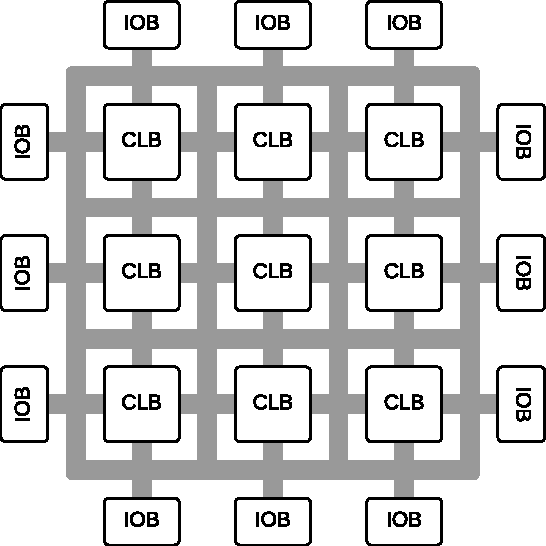
\includegraphics[width=0.30\textwidth]{figures/fpga}
    \caption{High-level block diagram of an FPGA. An array of configurable logic blocks (CLBs) and input/output blocks (IOBs) are connected by a network of interconnects.}
    \label{fig:fpga}
\end{figure}

FPGAs have been the subject of EHW research due to their reconfigurability, and several researchers have been successful in evolving working electronic circuits \cite{huelsbergen1998evolution, thompson1997evolved}.
However, the resulting circuits have often ended up using intrinsic properties of the silicon and been very sensitive to environmental changes.

The trouble with using modern FPGAs for EHW research is that some configuration bitstrings can destroy the FPGA \cite{ug380, xapp151}.
This means that the bitstring can not be used directly as the genotype without complicated tests to discard the dangerous bitstrings.
One solution to this problem is the sblock. \todo{does this sentence fit in here?}

\subsection{Sblock}

\begin{itemize}
    \item Haddow: \cite{haddow2000sblock}
    \item Basicly a configurable CA
    \item Virtual FPGA
    \item Add figure
\end{itemize}

\subsection{PCI Express}

The PCI Express interface was designed to tackle the arising trouble with clocked parallel buses like PCI.
The problem with such buses is that the clock speed can not be increased beyond a given threshold, as the slightly different lengths of the many wires causes data to arrive at slightly different times.
Reducing the clock period to less than the variation in arrival time means the data will become corrupted.
This problem is exacerbated with increasing bus size.

PCI Express is therefore based on serial communication over differential pairs (lanes \footnote{
        PCI Express operates in full duplex mode, which means that each lane has an independent differential pair in each direction.
        1, 2, 4, 8, 16 or 32 lanes are supported, but data is striped and thus still transmitted serially.
    }) without the need for a reference clock \cite{pcie}.
This allows an extremely fast clock speed compared to a parallel bus, and much greater bandwidth in total.
PCI Express consists of three layers; the physical layer, the data link layer and the transaction layer, structured as shown in \figurename~\ref{fig:pcie}.

\begin{figure}[!ht]
    \centering
    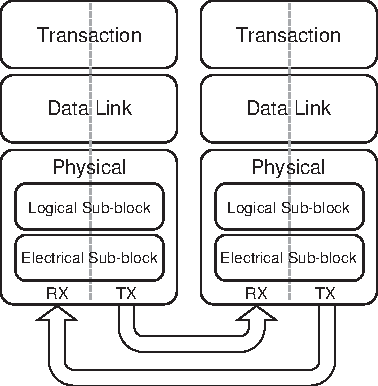
\includegraphics[width=0.25\textwidth]{figures/pcie}
    \caption{High-level diagram showing the layered structure of PCI Express. (Reprinted from \cite{pcie})}
    \label{fig:pcie}
\end{figure}

The transaction layers primary responsibility is the creation and parsing of transaction layer packets (TLPs).
TLPs are used to trigger events or start various transactions, most commonly to initiate read and write requests \footnote{
        Read and write requests are directed at one of up to six base address registers (BARs).
        They represent internal memory areas that can be anywhere from a few bytes to several gigabytes in size.
    }.
Most requests entail the return of a completion TLP containing the requested data or other information.
TLPs consists of multiple 32-bit double words (DW), where the first is a common header describing the type of packet.

The data link layer ensures integrity by adding error detection codes to outgoing TLPs and performing error detection and correction on incoming TLPs.
It is also responsible for retransmission if corruption occurs.

The physical layer is responsible for serialization and deserialization of the data stream.
Each byte is padded with two extra bits (8b/10b encoding) to allow clock recovery.

